\documentclass[../../monografia.tex]{subfiles}
\graphicspath{ {images/}{../images/}{../../images/} }

\begin{document}

\chapter{Used Tools}

\section{Main program development}
\subsection{C and C++ programming languages}
C and C++ are essential programming languages in embedded systems development due to their efficiency and control over hardware resources.

C was used not only for developing the firmware for the STM32 microcontroller (BluePill) but also for the hardware emulation. Its low-level capabilities allow precise control over microcontroller peripherals and were crucial for simulating the hardware's behavior.

C++ extends C with object-oriented features, making it ideal for more complex system architectures. In this project, C++ was utilized in the robotic simulation, especially within the ROS environment. Its object-oriented approach helped manage the complexity of the system, allowing better modularity and code organization, especially when dealing with ROS nodes and topics.

Thus, C was key in both the firmware development and hardware emulation, while C++ was primarily used for the simulation environment, leveraging its additional features for managing higher-level structures.

\subsection{CubeMX}

STM32CubeMX is a microcontroller configuration tool provided by STMicroelectronics. It was used for the initial configuration of the STM32F103C8T6 microcontroller, including generating the base project code and setting up peripherals such as UART, SPI, and GPIO. The tool simplified pin mapping and system parameter configuration, facilitating the integration between hardware and software.

\section{Microcontroller Emulation}
\subsection{QEMU}
QEMU \cite{QEMU_website_24} was used as the hardware emulator for the STM32F103C8T6 microcontroller. The specialized version for STM32 microcontrollers allowed for precise simulation of the microcontroller’s functionalities, particularly in emulating GPIO interfaces, which are essential for controlling external devices. QEMU enabled testing the firmware behavior without the need for physical hardware.

\subsection{ROS}

ROS \cite{ROS_website_24} was used as middleware for communication between the microcontroller emulation and the robotic environment simulation. Through ROS topics, the emulated GPIO input and output signals of the STM32 were sent and received, allowing the emulated microcontroller to interact seamlessly with the simulation environment.


\section{Simulation}
\subsection{Gazebo}

Gazebo was the main tool used for simulating the robotic environment. It allowed for testing the interactions of the microcontroller with the simulation in a visual and interactive manner, particularly in controlling actuators and reading sensor data. The integration between Gazebo, ROS, and the emulated microcontroller enabled a more realistic and efficient simulation of the overall robotic system.
\subsection{Blender}

Blender is an open-source 3D modeling and animation software widely used in various fields, including game development, visual effects, and architectural visualization. It provides a comprehensive suite of tools for modeling, sculpting, texturing, and rendering, making it a versatile choice for creating detailed 3D environments.

In this project, Blender was utilized to model the test environment for the robotic simulation. The detailed 3D models created in Blender were essential for accurately representing the physical environment in which the robot would operate. Once the modeling was completed, the environment was exported in a compatible format for integration with Gazebo, allowing for realistic simulation and interaction with the robot in the virtual world.

\section{Hardware development}
\subsection{Altium desing}

Altium Designer is a professional PCB (Printed Circuit Board) design software that was used to design a custom circuit board for the project. The PCB was designed to adapt the system for use in the real robot. Altium Designer offers a complete set of tools for schematic capture, PCB layout, and component management, making it ideal for creating custom hardware solutions.
\subsection{Multisim}

Multisim is an industry-standard software used for simulating electronic circuits. It allows for the creation and testing of circuit designs in a virtual environment, offering a wide range of tools for analyzing circuit behavior under different conditions. In this project, Multisim was utilized for initial testing of the hardware that was designed using Altium Designer. Before physically assembling the printed circuit board (PCB), simulations in Multisim helped validate the planned design, ensuring that key components and circuit configurations would function as expected when implemented in the real-world system.

\section{Hardware technologies}
\subsection{Robot Pionner 2}

The Pioneer 2 is a mobile robot platform developed by Adept MobileRobots (formerly ActivMedia Robotics). It is widely used in academic research and robotics education due to its robustness and flexibility in various applications such as navigation, mapping, and autonomous robotics. The Pioneer 2 is equipped with multiple sensors and interfaces, making it ideal for testing algorithms and embedded systems in real-world scenarios.

In this project, the Pioneer 2 was chosen as the physical robot for system validation. It was made available by POLI for use as the real robot platform.

% add robot pic

\subsection{Bluepill developement board}

The Blue Pill is a small, low-cost development board featuring the STM32F103C8T6 microcontroller, part of the STM32 family from STMicroelectronics. The board is highly popular in embedded systems projects due to its affordability, versatility, and relatively powerful ARM Cortex-M3 core. It comes equipped with 64 KB of flash memory, 20 KB of RAM, and operates at a frequency of 72 MHz, providing sufficient performance for a wide range of applications.

\subsection{Esp32 D1 Mini}

\clearpage

\begin{wrapfigure}{r}{5cm}
    \centering
    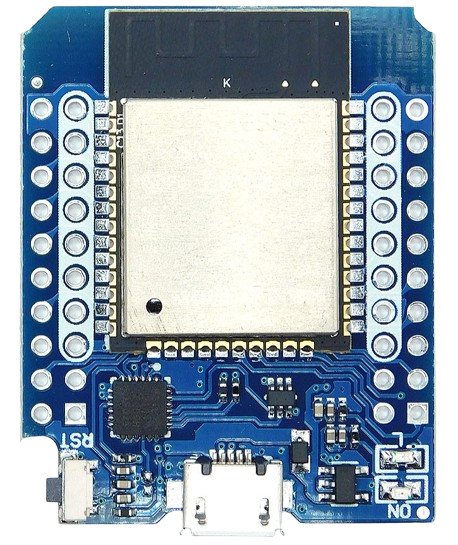
\includegraphics[width=4cm]{esp32d1mini-removebg.png}
    \caption{ESP32 D1 Mini}
    \label{fig: ESP32 D1 mini}
\end{wrapfigure}

The ESP32 \cite{esp32_2024} D1 Mini is a development board built around the ESP32 microcontroller from Espressif Systems. The board features dual-core processing with a 32-bit Tensilica LX6 microprocessor running at up to 240 MHz. It comes equipped with 4 MB of flash memory and 520 KB of SRAM, supporting some connectivity options, like Wi-Fi, classic Bluetooth, and BLE Bluetooth. These capabilities make the ESP32 D1 Mini an ideal choice for IoT applications, sensor networks, and embedded projects in general.


\end{document}

